\documentclass[conference]{IEEEtran}
\usepackage{cite}
\usepackage{url}
\usepackage[cmex10]{amsmath}
\usepackage{algorithm}
\usepackage{algpseudocode}
\usepackage{array}
\usepackage{mdwmath}
\usepackage{mdwtab}
\usepackage{eqparbox}
\usepackage{graphicx,subfigure}
\usepackage {epsfig}
\usepackage{fixltx2e}

\begin{document}

\title{JavaScript Profiling and Optimization on V8}

\author{
\IEEEauthorblockN{Yilin Zhang}
\IEEEauthorblockA{zylime@gmail.com}
\and
\IEEEauthorblockN{C. Vic Hu}
\IEEEauthorblockA{vic@cvhu.org}
}

\maketitle

\begin{abstract}

In this course project, we want to focus on the trace profiling and optimizations in the V8 JavaScript Engine used in Google Chrome. By learning from their existing compiling infrastructure and optimization processes, we hope to extract the key essence out of the works done the V8 open source community, and to apply the optimization techniques covered in our class. Ultimately, we want to study what it takes to build a super fast JavaScript engine in the industry, and to see if we can come up with some feasible ideas to make some enhancements.

\end{abstract}

\section{Introduction}



Although JavaScript is traditionally translated into byte code by an interpreter, more and more JavaScript Engines in modern browsers  are designed to compile directly into machine code. Our project will mainly focus on trace profiling\cite{Trace} in V8, and making constructive adjustments according to the optimization techniques we have learned in class. We will use the SunSpider JavaScript benchmark and the V8 benchmark to measure and compare the existing infrastructures, and make a sound analysis of the results. Our overall goal is to understand the common optimization procedures performed by modern JavaScript Engines, as well as the possible performance enhancements with the knowledge we've acquired from EE382V. 

In this paper, we will cover our motivations for doing this project, background information and detailed compilation processes about the V8 engine, profiling results, and comparisons to show the effectiveness of the optimizations done in V8.
%
%As we know internet riches people's life with new and quick information. At the same time people spend more and more timing browsing various websites. How to make the webpages response faster and save people's time becomes important. Infrastructure of cables and servers definitely play an important role, but compilation optimization\cite{Trace} and arrange the HTML tree\cite{Popularity} make difference when the infrastructure is unchangable.
%
%In this work, we will tackle both compilation optimization and arrangement of the HTML tree to accelerate the web response. We use TraceMonkey to help build the trace information and several optimization techniques are applied based on the trace structure. We analyze the web site popularity from the HTTP log file and then revise the HTTP tree based on the popularity.

%
\section{Motivation}
JavaScript has been widely used in web-based applications to increase richer interactions and visualizations \cite{mcduffie} since it was first supported by Netscape 2 beta back in 1995 \cite{jshistory}. In over fiften years, it has evolved into a variety of frameworks and libraries to enable a more interactive and dynamic web browsing experience \cite{ajax}, or even to build high-performance network programs \cite{node}. Besides its applications in web-based softwares, JavaScript has also gained its popularity from applications such as Adobe Flash, Dashboard widgets in Mac OSX, browser extensions, and web bookmarklets. Apart from its essential role in client-side interactions, JavaScript also became one of the mainstream server-side solutions in recent years\cite{node}. 

As the popularity of web-based applications and services increases, browser performance has become one of the major competitions in the industry. Since JavaScript is what makes modern web pages dynamic and interactive, how to optimize its compilation/interpretation is the key component to building fast and robust modern browsers. In the following two figures, we compared modern web browsers on two JavaScript benchmarks, including Chrome Canary, Chrome, Firefox, Safari, and Opera. In Fig.\ref{figure:v8_benchmark}, it was clear that both Chrome Canary (the latest beta release) and Chrome significantly outperformed any other competitors among all the test cases in the V8 benchmark suites. In Fig.\ref{figure:spider_benchmark}, although it became less obvious that Chrome was superior than its peers in the SunSpider benchmark, we can still see the dominance of V8 in general. V8 benchmark suite was provided by the same community who developed the V8 engine, which was mainly composed of , while SunSpider focused on utility performance such as text manipulation, encryption/decryption, data structure access, and common operations.

\begin{figure}[hbt!]	
	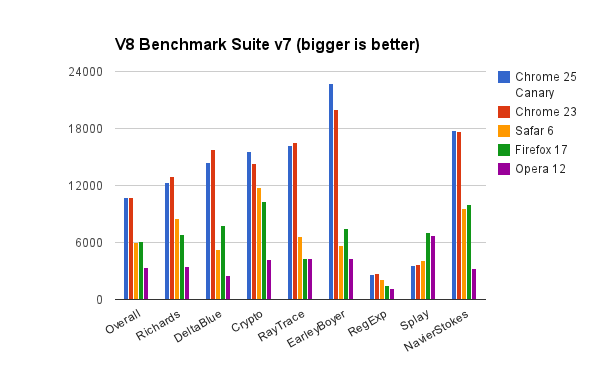
\includegraphics[width=0.5\textwidth]{figs/v8_benchmark.png}
	 \caption{ Testing results on the V8 Benchmark suite v7}
	 \label{figure:v8_benchmark}
\end{figure}

\begin{figure}[hbt!]	
	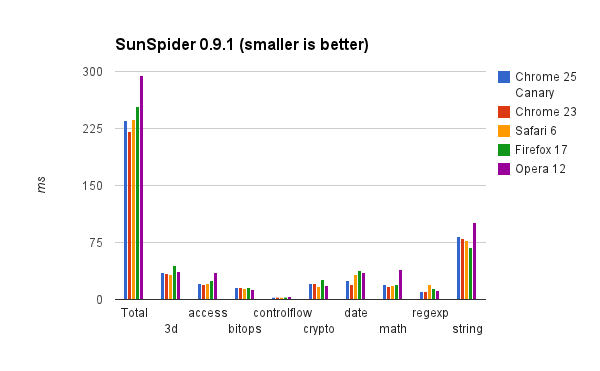
\includegraphics[width=0.5\textwidth]{figs/sunspider_benchmark.png}
	\caption{Testing results on the SunSpider Benchmark v0.9.1}
	\label{figure:spider_benchmark}
\end{figure}


\section{Background of V8 Engine}



\section{Approach}

JavaScript is slow mainly due to JavaScript programs are untyped, and then compiled and run on the fly. Dynamic compilation is a great complement to static one. But completely replacing the optimized-to-death static compilation with JIT will lose the performance. 
%
%

%%%%%%Prime Algorithm starts here%%%%%%%%%%%%%%%%%%%%%%%%%%%%%%%%%%%%%%%%%%%%%%%%%%%%%%%%%%%%%%%%%%%%

\begin{algorithm}[hbt!]
	\caption{\scriptsize{\emph{Calculate the 25000th Prime Number}}}
	 \label{algorithm:prime}
	 \begin{algorithmic}[1]
%		 \begin{scriptsize}			 
%\If {$i\geq maxval$}
%    \State $i\gets 0$
%\Else
%    \If {$i+k\leq maxval$}
%        \State $i\gets i+k$
%    \EndIf
%\EndIf
			\Require
			 \Ensure {The 25000th Prime Number P}
			 \State {Prime list PL = \{\}} 
			 \For {P = 1 to infinity}
			    \State {Flag = true}
			    \For{index = 1 to PL.size()}
			 	\If {P.mod(PL[i]) == 0}
			            \State {Flag = false}
			            \State {Continue}
			        \EndIf
			    \EndFor
			    \If {Flag == true}
			        \State {PL.push\_back(P)}
			        \If {PL.size() == 25000}
			            \Return {PL.back()}
			        \EndIf
			     \EndIf
			  \EndFor
%		\end{scriptsize}
	\end{algorithmic}
\end{algorithm}

%%%%%%%%%%%%%%%%%%%%%%%%%%%%%%%%%%%%%%%%%%%%%%%%%%%%%%%%%%%%%%%%%%%%%%%%%%%%%%%%%%%%%%%%%%%%%%%%%%

JavaScript is slower compared with other programming languages, such as C++. Before applying the optimization to the compilation of JavaScript code, we use one example to demonstrate how slow JavaScript is compared with C++. 

The example we use here is to calculate the 25000th prime number\cite{googleIO}. The overall algorithm of calculating the 25000th prime number is illustrated in Algorithm\ref{algorithm:prime}.
The C++ code implementing the algorithm is in the Fig.\ref{figure:prime_cplusplus} while the JavaScript version is in the Fig.\ref{figure:prime_JavaScript}.

\section{Results}
\begin{figure}[hbt!]
    \centering
        \subfigure[]{
            \label{figure:prime_cplusplus}
            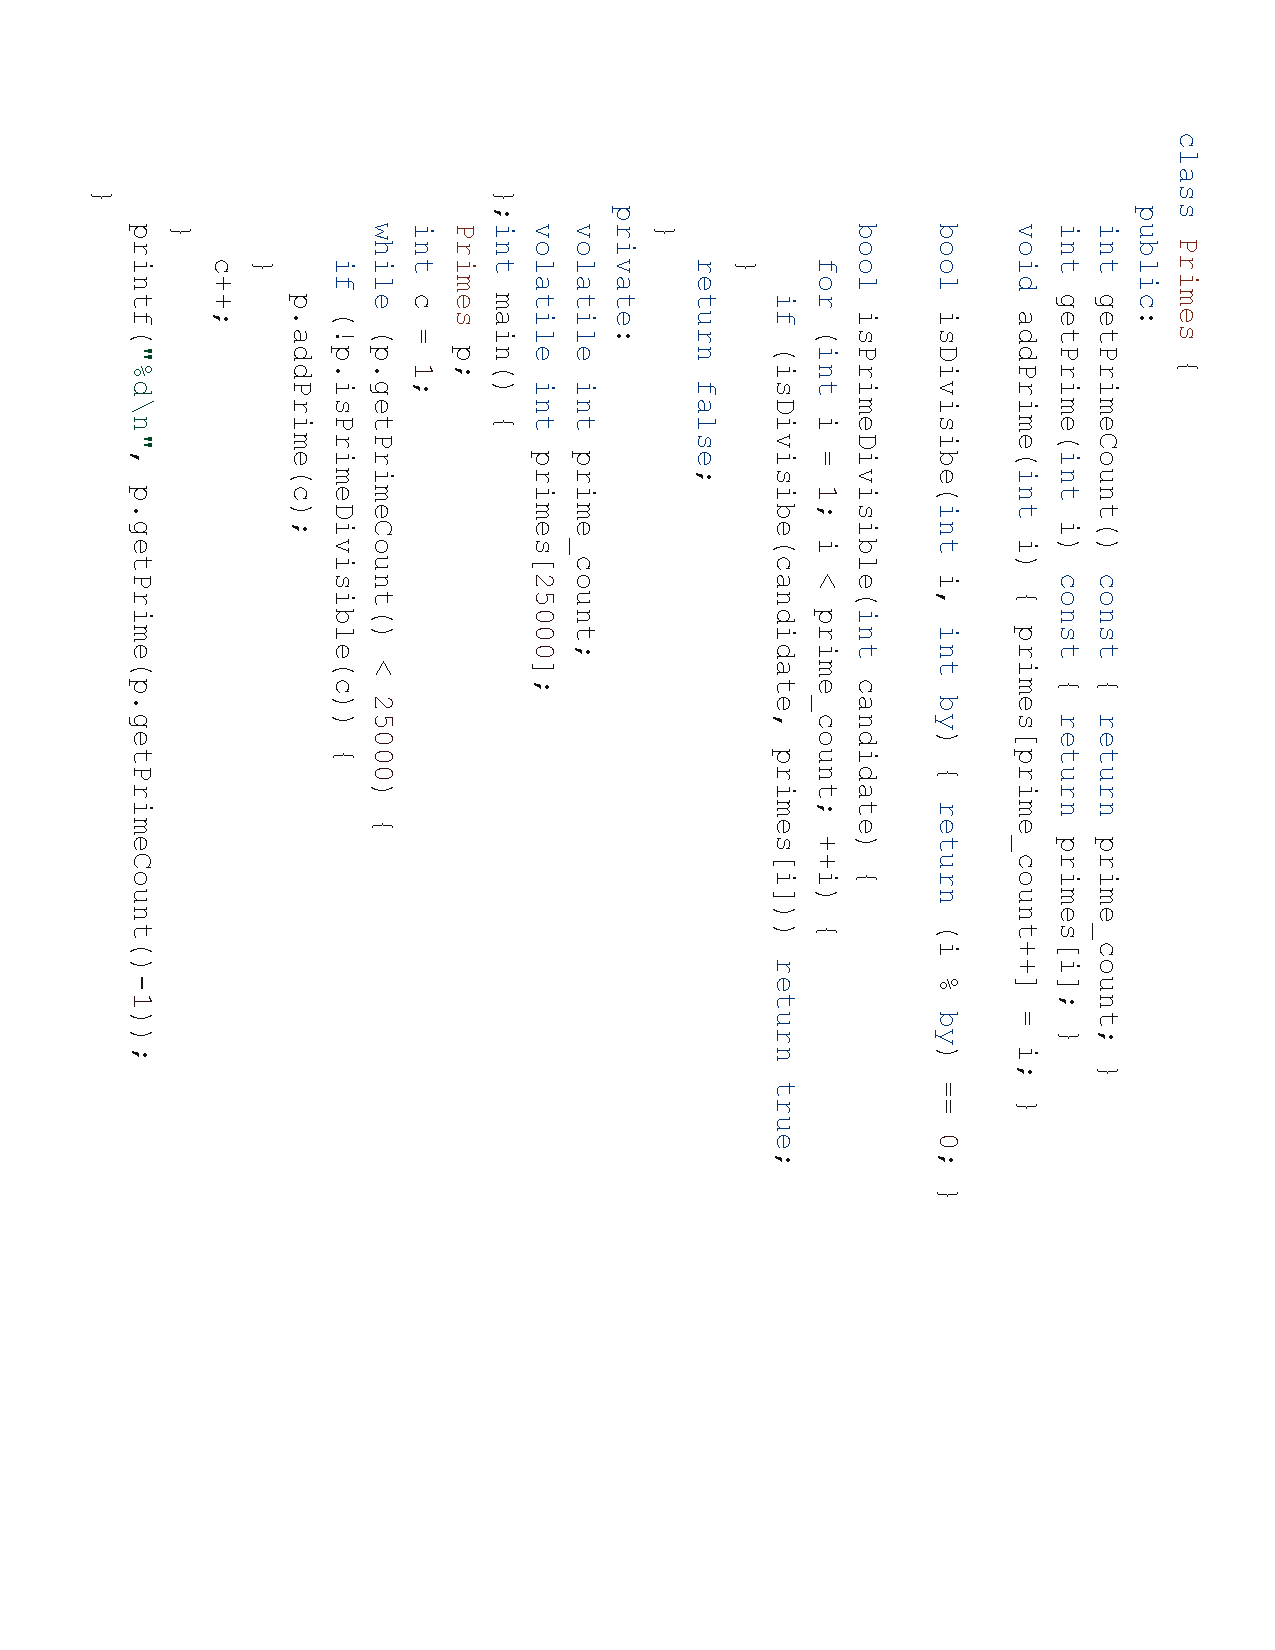
\includegraphics[width=0.64\textwidth]{figs/prime_cplusplus}
        }
        \subfigure[]{
           \label{figure:prime_JavaScript}
           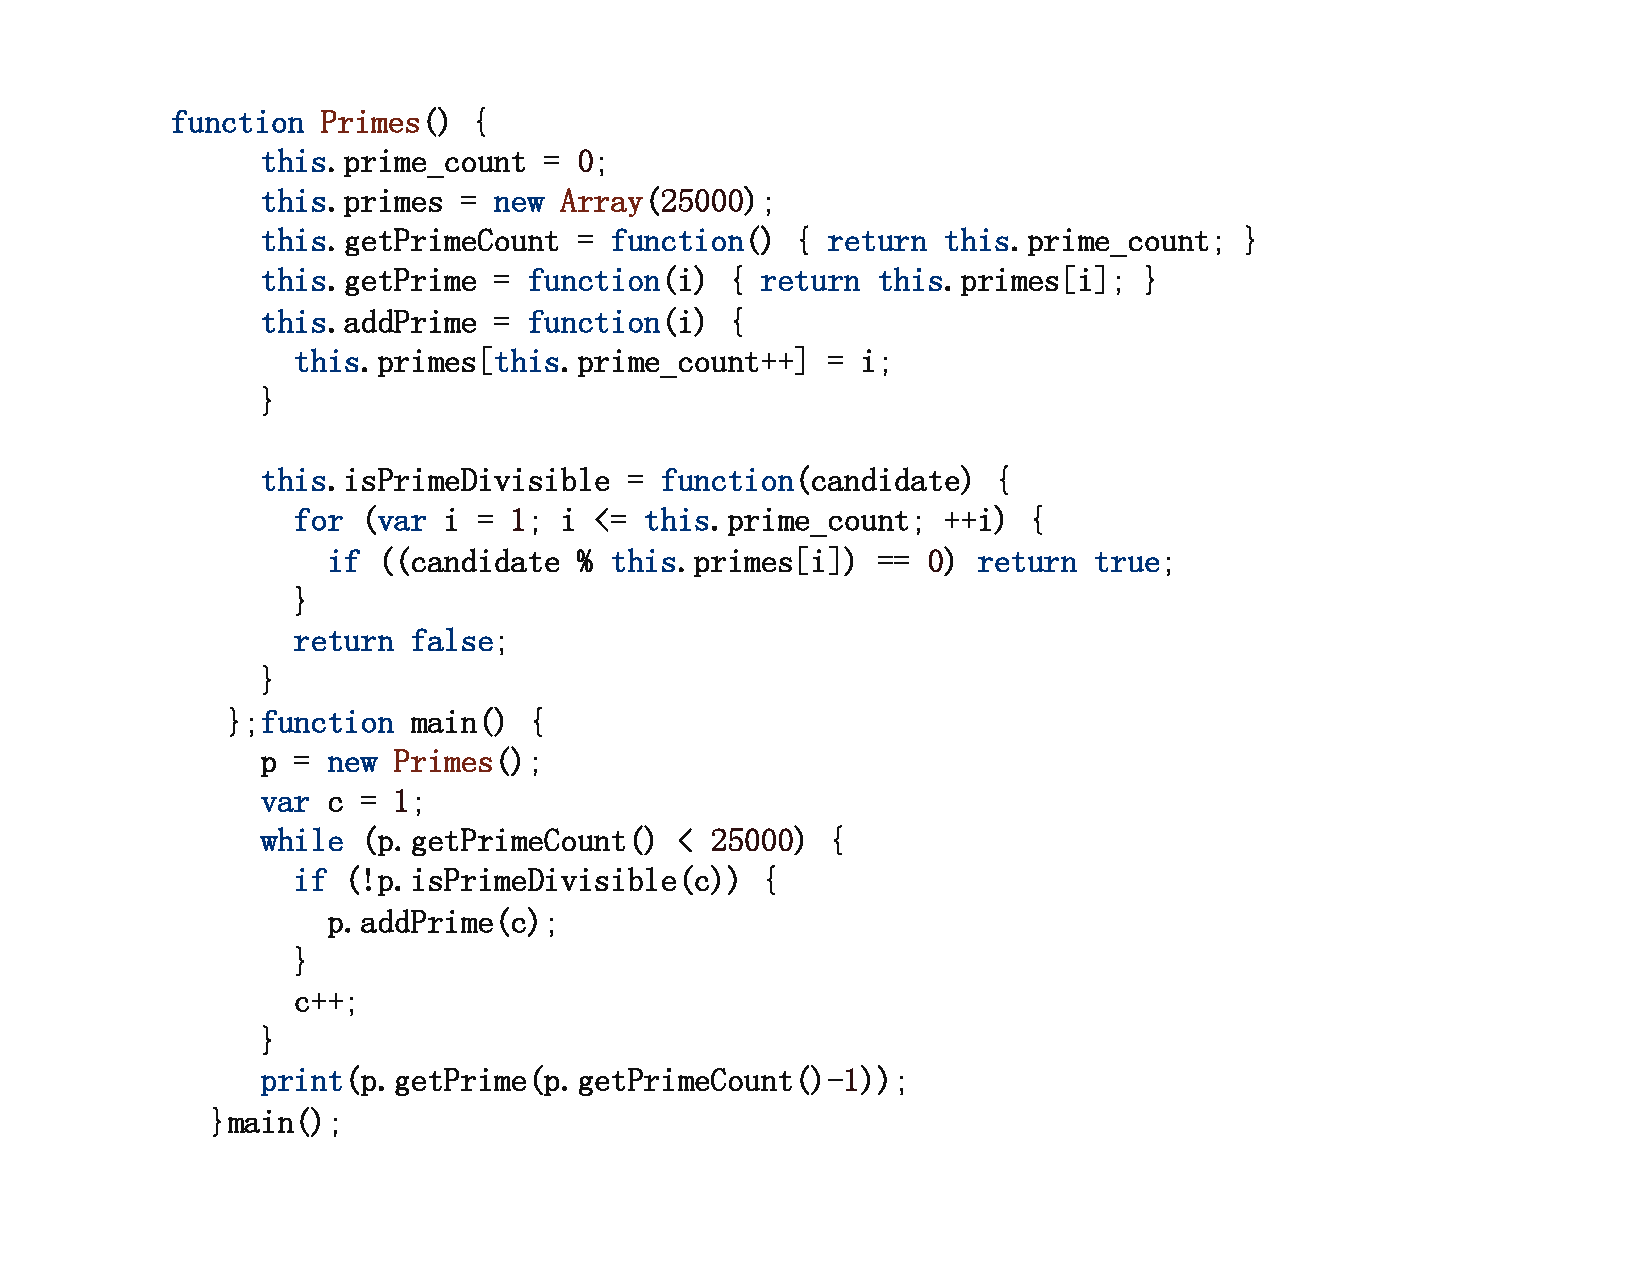
\includegraphics[width=0.64\textwidth]{figs/prime_JavaScript}
        }
    \caption{(a) is the C++ code of calculating the 25000th prime number (b) is the JavaScript code for 25000th prime number.}
	\label{figure:prime}
 \end{figure}

\section{Conclusion}

\section{Acknoledgment}



%
%
%
%\section{Approach}
%
%
%

%
%\section{Results}
%
%\subsection{Experimental Framework}
%
%
%
%\subsection{Data}
%
%
%
%
%
%\begin{table}[h]
%% increase table row spacing, adjust to taste
%\renewcommand{\arraystretch}{1.3}
%\caption{There is no period in a table caption}
%\label{table_example}
%\centering
%% Some packages, such as MDW tools, offer better commands for making tables
%% than the plain LaTeX2e tabular which is used here.
%\begin{tabular}{|c||c|}
%\hline
%One & Two\\
%\hline
%Three & Four\\
%\hline
%\end{tabular}
%\end{table}
%\renewcommand{\arraystretch}{1}
%
%\section{Related Work}
%
%
%
%\section{Conclusion}
%
%
%
%\section*{Acknowledgment}


\begin{thebibliography}{1}

\bibitem{jshistory}
Eich, Brendan. "JavaScript at ten years." ACM SIGPLAN Notices. Vol. 40. No. 9. ACM, 2005.
\bibitem{mcduffie}
McDuffie, Tina. JavaScript Concepts \& Techniques: Programming Interactive Web Sites. Franklin Beedle \& Associates, 2003.
\bibitem{ajax}
Serrano, Nicol�s, and Juan Pablo Aroztegi. "Ajax frameworks in interactive web apps." Software, IEEE 24.5 (2007): 12-14.
\bibitem{node}
Tilkov, Stefan, and Steve Vinoski. "Node. js: Using JavaScript to build high-performance network programs." Internet Computing, IEEE 14.6 (2010): 80-83.
%\bibitem{IEEEhowto:kopka}
%H.~Kopka and P.~W. Daly, \emph{A Guide to \LaTeX}, 3rd~ed.\hskip 1em plus
%  0.5em minus 0.4em\relax Harlow, England: Addison-Wesley, 1999.
\bibitem{Trace}
Jungwoo Ha and Mohammad R. Haghighat and Shengnan Cong, A concurrent trace-based just-in-time compiler for javascript, Tech Report, 2009
\bibitem{Popularity}
John Garofalakis and Panagiotis Kappos and Dimitris Mourloukos, Web site optimization using page popularity, Internet Computing, 1999
\bibitem{node}
"Why Everyone Is Talking About Node." Jolie O'Dell. Mashable, Inc., Web. 10 Mar. 2011.
\bibitem{googleIO}
"Breaking the JavaScript Speed Limit with V8", Google I/O, 2012

\end{thebibliography}




% that's all folks
\end{document}
